\chapter{PENDAHULUAN}
\section{Latar Belakang}
Badan Pusat Statistik (BPS) merupakan suatu lembaga pemerintah non-departemen yang bertanggung jawab dalam penyediaan statistik dasar. Dalam peranannya sebagai penyedia data, BPS melakukan pengumpulan data dengan 2 (dua) metode : primer dan sekunder. Pengumpulan data primer berarti BPS secara mandiri mengumpulkan data dengan menggunakan metode wawancara langsung dengan responden, baik responden individu, rumah tangga, maupun perusahaan. Sementara pengumpulan data sekunder berarti BPS memperoleh data dari pihak lain.

Dalam melakukan kegiatan perstatistikan, yang selanjutnya merujuk kepada pengumpulan data primer, BPS merujuk kepada \textit{General Statistical Business Process Model} (GSBPM) ~\cite{_gsbpm_????}, yang merupakan suatu standard arsitektur bisnis kegiatan perstatistikan yang dirumuskan oleh \textit{United Nations Economic Commission for Europe} (UNECE). Dalam GSBPM, \textit{Business Process} Statistik dibagi menjadi 7 (tujuh) phase : \textit{Specify Needs}, \textit{Design}, \textit{Build}, \textit{Collect}, \textit{Process}, \textit{Analyze}, \textit{Disseminate}, \textit{Evaluate}, dimana masing-masing phase dipecah menjadi beberapa sub-proses.

\begin{figure}
    \centering
    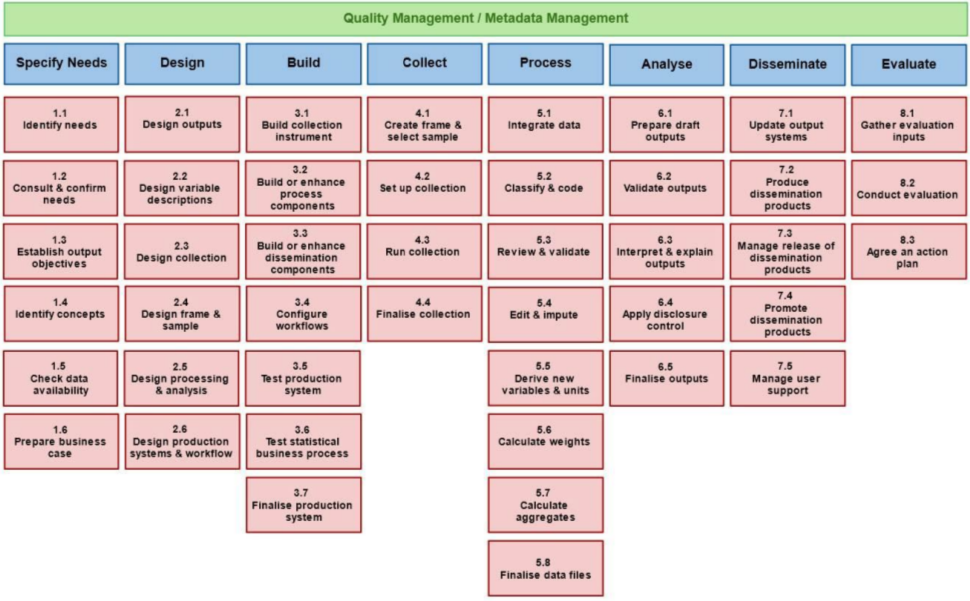
\includegraphics[height=6cm]{images/GSBPM}
    \caption{\textit{Statistical Business Process Phases} dalam GSBPM}
    \label{fig:gsbpm}
\end{figure}

Pengumpulan dan pengolahan data dalam GSBPM tercakup dalam 3 (tiga) fase, yaitu : \textit{Collect Phase}, \textit{Process Phase}, dan \textit{Analyze Phase}. \textit{Collect phase} adalah fase dimana semua informasi (data dan metadata) dikumpulkan dengan menggunakan beberapa metode pengumpulan (termasuk ekstraksi dari register dan database statistik, administratif, maupun yang lain), dan memuatkannya ke dalam suatu \textit{environment} untuk pemrosesan lebih lanjut. \textit{Process phase} adalah fase dimana data dibersihkan dan dipersiapkan untuk tahap berikutnya, \textit{analysis phase}. \textit{Collect phase} dan process phase dapat dilakukan secara berulang dan paralel. Fase terakhir sebelum data siap untuk didesiminasikan adalah \textit{analyze phase}. Pada tahap \textit{analyze phase}, data ditransformasikan kedalam bentuk \textit{statistical output} yang disesuaikan dengan kebutuhan (\textit{fit for purpose}).

Kondisi saat ini, \textit{process phase} dan \textit{analyze phase} merupakan tahapan yang memiliki ketergantungan akan Teknologi Informasi dan Komunikasi (TIK) yang sangat besar. \textit{Process phase} merupakan tahapan dimana dilakukan input data hasil pendataan lapangan dari format kuesioner ke dalam format digital, termasuk didalamnya pengkodean, imputasi, validasi, dan penghitungan penimbang. Sementara \textit{analyze phase} memerlukan keterlibatan software analisis yang membantu mentransformasikan data menjadi sebuah informasi. Adapun \textit{collect phase}, meskipun saat ini masih menggunakan pengumpulan data dengan mengadopsi \textit{paper questionaire}, tetapi kedepannya akan dilakukan transformasi dengan menggunakan metode \textit{Computer Assisted Personal Interviewing} (CAPI)\footnote{Keterangan Dr. Said Mirza Pahlevi, M.Eng., Kepala Subdirektorat Pengembangan Basis Data, 24 Februari 2016}, meskipun feasibility-nya belum pernah diujicobakan\footnote{Keterangan Dr. Muchammad Romzi, Kepala Subdirektorat Pengembangan Model Statistik, 4 Maret 2016}. 

Penggunaan metode CAPI dalam pengumpulan data yang dilakukan BPS, sedikit banyak akan mengubah paradigma pengumpulan dan pengolahan data yang selama ini telah berjalan. Pengumpulan dan pengolahan data yang selama ini merupakan dua buah tahapan yang terpisah, dengan diterapkannya CAPI maka beberapa sub-proses dari \textit{process phase}, seperti pengkodean dan validasi, dapat dilakukan secara terintegrasi dengan pengumpulan data. Metode CAPI sebenarnya bukanlah sebuah hal yang baru. Metode ini sudah ada sejak beberapa dekade terakhir ~\cite{_redesigning_????}. Bahkan sebuah penelitian yang dilakukan oleh Gary Klein dkk menyatakan pengumpulan data dengan menggunakan metode CAPI berpotensi terjadi bias, terutama dalam akurasi, \textit{completeness}, dan \textit{item omission} ~\cite{klein_bias_1996}. Akan tetapi, dengan semakin berkembangnya teknologi \textit{mobile computing} yang dipadukan dengan penggunaan \textit{Web service} ~\cite{tergujeff_mobile_2007}, maka potensi bias dapat dikurangi dengan merancang beberapa \textit{web service} yang digunakan untuk menvalidasi hasil pendataan.

Implementasi pengumpulan data dengan menggunakan CAPI yang terintegrasi dengan penggunaan \textit{Web service} bukanlah tanpa kendala. Petugas pengumpulan data harus berpindah-pindah dari satu lokasi pendataan ke lokasi yang lain untuk mengunjungi responden. Dikarenakan keterbatasan infrastruktur seperti telekomunikasi dan daya tahan baterai \textit{device}, seringkali sulit bagi \textit{device} untuk selalu terhubung dengan \textit{Web service}. \textit{Device} dapat kapan saja berubah dari \textit{connected node} menjadi \textit{disconnected node} dan sebaliknya. 

\begin{figure}
    \centering
    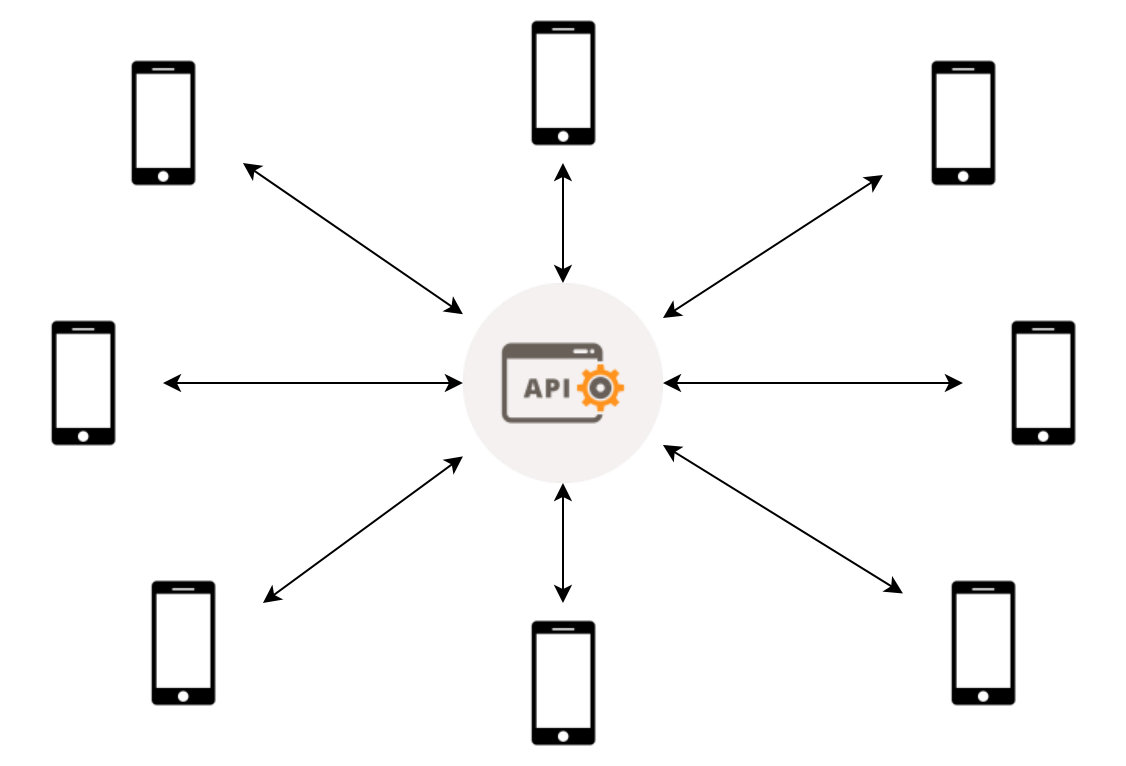
\includegraphics[height=6cm]{images/CAPI-Ilustration}
    \caption{Ilustrasi CAPI}
    \label{fig:capi-ilustration}
\end{figure}

Brian DeRenzi dkk telah melakukan penelitian tentang cara pengumpulan data berbasis \textit{mobile phone} pada lingkungan yang \textit{highly disconnected} ~\cite{derenzi_reliable_2007} dengan menggunakan \textit{CAM Framework}. \textit{CAM framework}~\cite{parikh_designing_2006} terbukti dapat digunakan dalam pengumpulan data dalam lingkungan yang \textit{disconnected}, dan setelah device kembali ke \textit{connected environment}, data yang terkumpul akan terupload ke server. Akan tetapi \textit{CAM framework} memiliki kelemahan, antara lain : 1) CAM berbasis \textit{fix-length text-based input}, yang membuatnya tidak cocok digunakan untuk pengumpulan data yang berbasis \textit{data-intensive}; 2) Tidak terdapat \textit{conflict resolution}, sehingga masih memungkinkan dua device atau lebih mengeksekusi data yang sama. Sementara itu, Takdir dkk mengusulkan penggunaan pola terdistribusi berbasis SOA untuk meningkatkan kinerja sistem yang bersifat data-intensif ~\cite{takdir_multi-layer_2014}. Penggunaan pola terdistribusi disini mencakup \textit{workflow} (\textit{Web service}) maupun \textit{data-service}. Mekanisme yang digunakan dalam perancangan service pola terdistribusi mencakup 3 (tiga) hal : sinkronisasi, replikasi, dan \textit{routing}. \textit{Composite application} yang dijalankan pada sisi \textit{client} akan melakukan replikasi data maupun \textit{Web service}, kemudian data dan \textit{Web service} tersebut digunakan secara lokal. Sementara itu, untuk menjamin konsistensi data, Takdir dkk mengakomodir mekanisme \textit{sinkronisasi}.

\begin{figure}
    \centering
    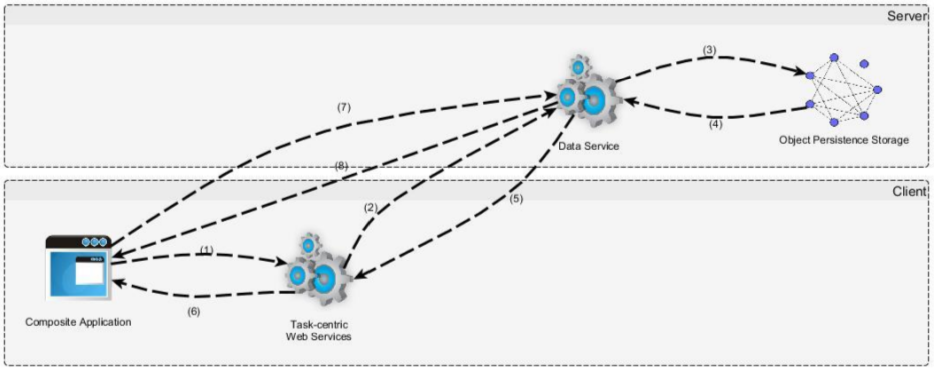
\includegraphics[height=5cm]{images/Takdir-Distributed-SOA}
    \caption{Skema Usulan, Takdir}
    \label{fig:takdir-soa}
\end{figure}

Berdasarkan hasil pengujian, pola distribusi berbasis SOA usulan Takdir dkk terbukti mampu memberikan hasil yang lebih baik, dengan penggunaan \textit{resource} CPU dan memory yang lebih rendah. Akan tetapi, lingkup perancangan dan pengujian sistem hanya terbatas pada perangkat komputer (\textit{desktop} maupun \textit{laptop}). Pada pola terdistribusi, usulan Takdir dkk, \textit{client} perlu untuk melakukan replikasi data maupun \textit{workflow} yang berupa \textit{Web service} agar dapat berjalan. Sementara pada pendataan data berbasis CAPI, perangkat yang digunakan adalah \textit{mobile device}, yang mempunyai arsitektur maupun \textit{resource} yang berbeda jika dibandingkan dengan komputer. Proses replikasi data data \textit{workflow} bisa menjadi sesuatu yang \textit{challenging} atau bahkan sulit dilakukan semenjak \textit{mobile device} bukanlah sesuatu yang umum digunakan sebagai \textit{service provider}.	Oleh karena itu, penelitian ini akan berfokus kepada perancangan desain dan implementasi sistem terdistribusi yang  dapat diimplementasikan pada perangkat \textit{mobile}.

\section{Rumusan Masalah}
Berdasarkan uraian latar belakang permasalahan diatas, maka dapat dirumuskan suatu permasalahan penelitian yaitu bagaimana merancang desain dan implementasi sistem terdistribusi pada perangkat \textit{mobile}.

\section{Tujuan Penelitian}
Tujuan utama dari penelitian ini adalah untuk merancang sebuah desain dan implementasi sistem terdistribusi pada perangkat \textit{mobile}. Adapun tujuan khusus penelitian ini adalah :
\begin{itemize}
\item Merancang sistem terdistribusi untuk perangkat \textit{mobile} yang mendukung kondisi \textit{connection-full} maupun \textit{connection-less},
\item Menganalisis kompatibilitas \textit{mobile device} yang memenuhi spesifikasi rancangan sistem,
\item Melakukan ujicoba atas desain dan implementasi sistem,
\item Menganalisis dan mengevaluasi hasil ujicoba sistem.
\end{itemize}

\section{Batasan Masalah}
Batasan masalah dalam penelitian ini adalah :
\begin{itemize}
\item Penelitian ini hanya berfokus pada desain dan implementasi sistem pada \textit{mobile device},
\item \textit{Mobile device} yang digunakan sebagai bahan penelitian terbatas hanya \textit{mobile device} dengan sistem operasi \textit{Android},
\item Perancangan GUI hanya digunakan sebagai bahan uji coba, dan bukan termasuk ke dalam poin inti penelitian.
\end{itemize}


